\documentclass{article}

\usepackage[utf8]{inputenc}
\usepackage{graphicx}
\usepackage{amsmath}
\usepackage{amsfonts}
\usepackage{amssymb}
\usepackage{comment}
\usepackage{gensymb}
\usepackage{geometry}
\usepackage{float}
\usepackage{caption}
\usepackage{subcaption}
\usepackage{listings}
\usepackage{enumitem}

\geometry{a4paper, margin=1in}

\lstset{
    basicstyle=\ttfamily\small,
}

\title{CSCE 312 Lab 5}
\author{Kevin Lei}

\date{March 31, 2024}


\begin{document}

\maketitle

\section*{Problem 1}

\begin{figure}[H]
    \centering
    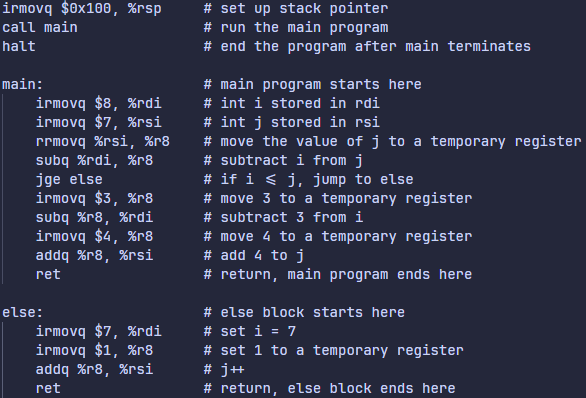
\includegraphics[width=0.6\textwidth]{../images/prob1_code.png}
    \caption{Y86-64 code for Problem 1}
\end{figure}

Note: \texttt{int i} stored in \texttt{\%rdi}, \texttt{int j} stored in \texttt{\%rsi}

\begin{figure}[H]
    \centering
    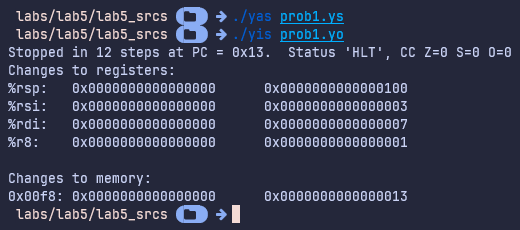
\includegraphics[width=0.6\textwidth]{../images/prob1_out1.png}
    \caption{Output for Problem 1 with \texttt{i = 1}, \texttt{j = 2}}
\end{figure}

\begin{figure}[H]
    \centering
    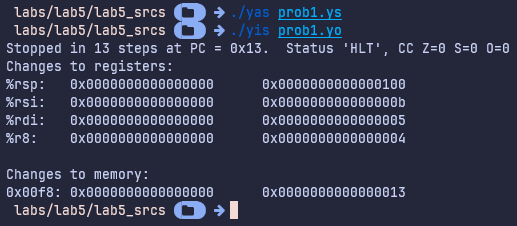
\includegraphics[width=0.6\textwidth]{../images/prob1_out2.png}
    \caption{Output for Problem 1 with \texttt{i = 8}, \texttt{j = 7}}
\end{figure}

\section*{Problem 2}

\begin{figure}[H]
    \centering
    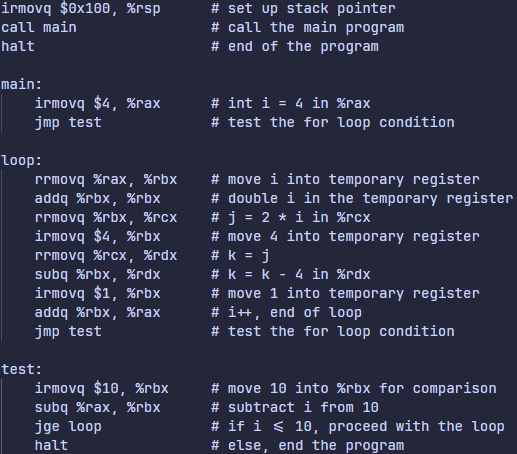
\includegraphics[width=0.6\textwidth]{../images/prob2_code.png}
    \caption{Y86-64 code for Problem 2}
\end{figure}

Note: \texttt{int i} stored in \texttt{\%rax}, \texttt{int j} stored in \texttt{\%rcx}, and \texttt{int k} stored in \texttt{\%rdx}.
Initial values of \texttt{j} and \texttt{k} do not matter, since they are both always overwritten by \texttt{i * 2} and \texttt{j - 4} (in other words \texttt{i * 2 - 4}) respectively.

\begin{figure}[H]
    \centering
    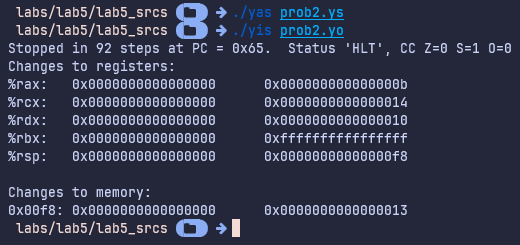
\includegraphics[width=0.6\textwidth]{../images/prob2_out.png}
    \caption{Output for Problem 2}
\end{figure}

\section*{Problem 3}

\begin{minipage}{0.5\textwidth}
    \begin{figure}[H]
        \centering
        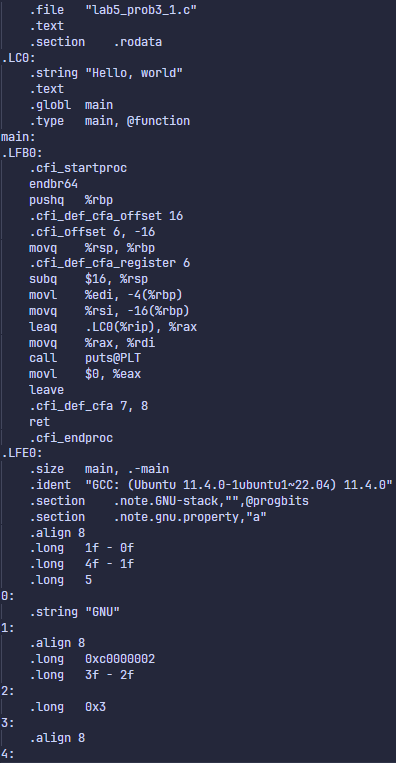
\includegraphics[width=0.9\textwidth]{../images/prob3_code1.png}
        \caption{x86-64 code for \texttt{lab5\_prob3\_1.c}}
    \end{figure}
\end{minipage}
\begin{minipage}{0.5\textwidth}
    \begin{figure}[H]
        \centering
        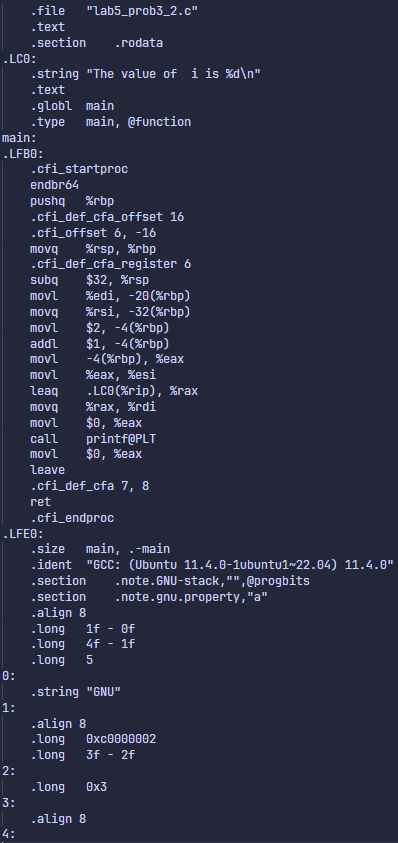
\includegraphics[width=0.9\textwidth]{../images/prob3_code2.png}
        \caption{x86-64 code for \texttt{lab5\_prob3\_2.c}}
    \end{figure}
\end{minipage}

\vspace{0.5cm}

The first program, \texttt{lab5\_prob3\_1.c}, just prints "Hello, world" to the console. 
Its x86-64 assembly equivalent starts with various directives and defines \texttt{.LC0} as the string "Hello, world", which will be accessed later.
Then, in the main function, it sets up the stack frame with \texttt{pushq \%rbp} and \texttt{movq \%rsp, \%rbp}.
The function arguments \texttt{argc} and \texttt{argv} get pushed to the stack with \texttt{movl \%edi, -4(\%rbp)} and \texttt{movq \%rsi, -16(\%rbp)},
even though they are not used in the program.
Finally, we get to the most important part of the program, which is the printing of "Hello, world" to the console.
The address of the "Hello, world" string is loaded into \texttt{\%rax} with \texttt{leaq .LC0(\%rip), \%rax}, and then the address is passed to \texttt{puts} with \texttt{movq \%rax, \%rdi} and \texttt{call puts@PLT}.
The \texttt{puts} function is what actually prints the string to the console.
Then, the program sets the return value to 0 with \texttt{movl \$0, \%eax} and exits with \texttt{leave} and \texttt{ret}.
The rest of the code is irrelevant to the program's functionality, and is just information for the compiler and linker.

The second program, \texttt{lab5\_prob3\_2.c}, declares an integer \texttt{i} and initializes it to 2, increments it by 1, and then prints it to the console.
The code is very similar to the first program, but with some minor differences.
Like the first program, it sets up the stack frame and function arguments and includes similar information for the compiler and linker.
Also, it declares the string \texttt{"The value of i is \%d\textbackslash n"} at \texttt{.LC0}.
In the function body, the integer \texttt{i} is declared and initialized to 2 with \texttt{movl \$2, -4(\%rbp)}
and then incremented with \texttt{addl \$1, -4(\%rbp)}.
The value of \texttt{i} is first loaded into \texttt{\%eax} with \texttt{movl -4(\%rbp), \%eax} and then to \texttt{\%esi} with \texttt{movl \%eax, \%esi}.
This was just to prepare the value of \texttt{i} to be printed with the \texttt{printf} function.
Finally, the address of the string is loaded into \texttt{\%rdi} with \texttt{leaq .LC0(\%rip), \%rax} and \texttt{movq \%rax, \%rdi}, and then \texttt{printf} is called with \texttt{call printf@PLT}.

\section*{Problem 4}
The main difference between \texttt{lab5\_prob3\_1.c} and \texttt{lab5\_prob4.c} is the way that the "Hello world" string is printed.
We can see from the C source code that \texttt{lab5\_prob3\_1.c} calls \texttt{printf()} directly in the main function, while \texttt{lab5\_prob4.c} calls a function \texttt{print\_hello()} that calls \texttt{printf()}.
In the assembly generated, the effective address of the string "Hello, world" is loaded into \texttt{\%rax} and moved into \texttt{\%rdi}, and then \texttt{call puts@PLT} is called, which effectively prints the string to the console.
In the code for \texttt{lab5\_prob4.c}, the corresponding assembly code calls \texttt{call print\_hello} in the main directive, and the \texttt{print\_hello} function uses the same logic as \texttt{lab5\_prob3\_1.c} to print the string to the console.

\section*{Problem 5}
\begin{minipage}{0.5\textwidth}
    \begin{figure}[H]
        \centering
        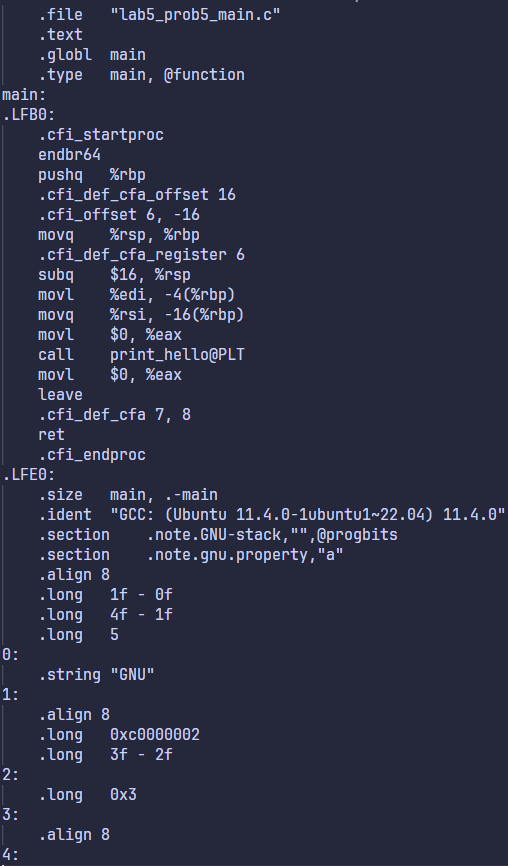
\includegraphics[width=0.9\textwidth]{../images/prob5_code1.png}
        \caption{Assembly generated from main code}
    \end{figure}
\end{minipage}
\begin{minipage}{0.5\textwidth}
    \begin{figure}[H]
        \centering
        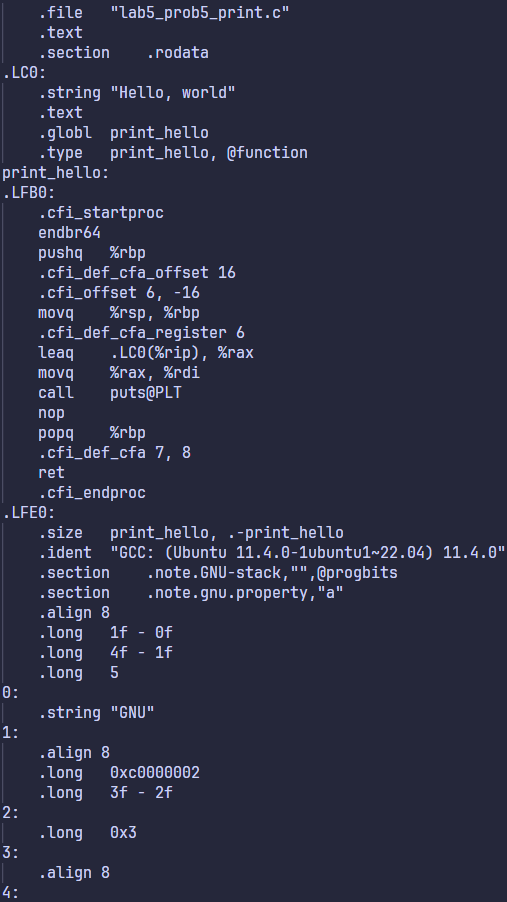
\includegraphics[width=0.9\textwidth]{../images/prob5_code2.png}
        \caption{Assembly generated from print function}
    \end{figure}
\end{minipage}

\begin{figure}[H]
    \centering
    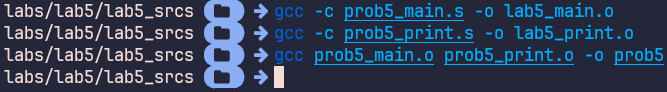
\includegraphics[width=0.6\textwidth]{../images/prob5_compile.png}
    \caption{Generating object files and linking them together}
\end{figure}

The difference between the assembly codes generated for this problem and the previous problem is that the \texttt{print\_hello()} function is now defined in a separate file, but the functionality and implementation of the function remain the same.
Both codes have a main directive that calls the \texttt{print\_hello()} function, and both \texttt{print\_hello()} functions load the address of the string "Hello, world" into \texttt{\%rax} and then move it into \texttt{\%rdi} before calling \texttt{puts@PLT}.


\section*{Problem 6}

\begin{figure}[H]
    \centering
    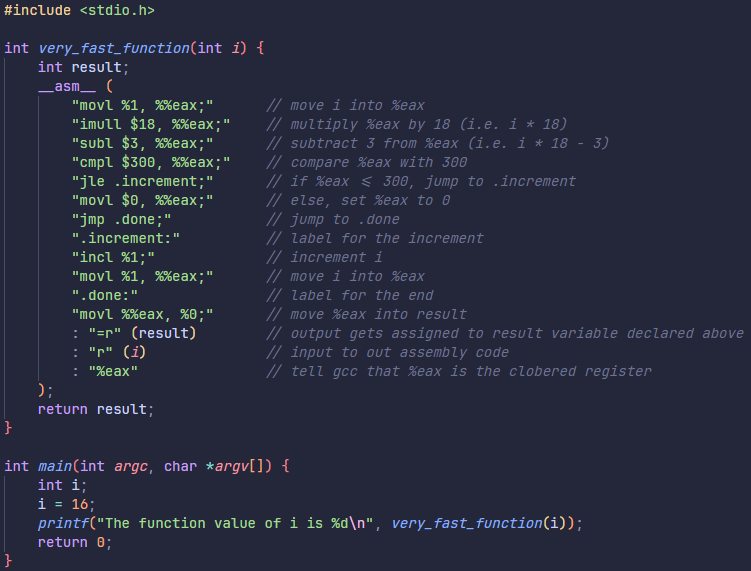
\includegraphics[width=0.8\textwidth]{../images/prob6_code.png}
    \caption{\texttt{very\_fast\_function()} rewritten with inline assembly}
\end{figure}

\begin{figure}[H]
    \centering
    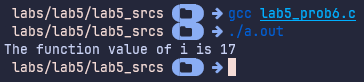
\includegraphics[width=0.5\textwidth]{../images/prob6_out.png}
    \caption{Compiling and running \texttt{lab5\_prob6.c}}
\end{figure}

\end{document}